\documentclass[12pt]{article}

% TEMPLATE DEFAULT PACKAGES
\usepackage{amssymb,amsmath,amsfonts,eurosym,geometry,ulem,graphicx,color,setspace,sectsty,comment,natbib,pdflscape,array,adjustbox}

% ADDED PACKAGES FOR THIS MANUSCRIPT
\usepackage{palatino,newtxmath,multirow,titlesec,threeparttable,tabu,booktabs,titlesec,threeparttable,mathtools,bm,bbm,subcaption,pdflscape,tcolorbox,mathrsfs}
% endfloat,

\usepackage{afterpage}
\usepackage[hyphens]{url}
\usepackage[margin=1cm]{caption}

\usepackage[draft]{hyperref}
\newcommand{\tim}{$\,\times\,$}
% FIGURES & TABLES CAPTION STYLING
\captionsetup[figure]{labelfont={bf},name={Figure},labelsep=period}
\captionsetup[table]{labelfont={bf},name={Table},labelsep=period}

% SECTION TITLE SETTINGS
\titlelabel{\thetitle.\enskip}
\titleformat*{\section}{\large\bfseries}
\titleformat*{\subsection}{\normalsize\bfseries}

% COLUMN TYPES
\newcolumntype{L}[1]{>{\raggedright\let\newline\\\arraybackslash\hspace{0pt}}m{#1}}
\newcolumntype{C}{>{\centering\arraybackslash}p{5.2em}}
\newcolumntype{D}{>{\centering\arraybackslash}p{5em}}
\newcolumntype{R}[1]{>{\raggedleft\let\newline\\\arraybackslash\hspace{0pt}}m{#1}}


% MARGINS AND SPACING
\normalem
\geometry{left=1.1in,right=1.1in,top=1.0in,bottom=1.0in}
\setlength{\parskip}{2.5pt}

% SPECIAL CELL 
\newcommand{\specialcell}[2][c]{%
	\begin{tabular}[#1]{@{}l@{}}#2\end{tabular}}

% NO INDENT ON FOOTNOTES
\usepackage[hang,flushmargin]{footmisc}

\begin{document}



% \vspace{0mm}
% \begin{table}[h!]
% \centering
% \caption{Housing Project Areas Description}\label{table:projectdescriptives}
% \vspace{0mm}
% \begin{tabular}{l*{1}{cccccc}}
% \toprule
%   & \multicolumn{2}{c}{\textbf{All}}& \multicolumn{2}{c}{\textbf{Greenfield}}  & \multicolumn{2}{c}{\textbf{In-Situ}}   \\
%   &Const. & Unconst. &Const. & Unconst.   & Const. & Unconst. \\
% \midrule
%  Number of Projects  & 172  & 145  & 43  & 20  & 27  & 29  \\ 
 Area (km2)  & 1.17  & 1.16  & 1.72  & 2.42  & 1.50  & 0.88  \\ 
 Median Construction Yr.  & 2006  & 2006  & 2006  & 2005  & 2004  & 2006  \\ 
 Delivered Houses  & 374  & 11  & 568  & 24  & 702  & 20  \\ 
 House Price in 1 km (R$^\dagger$)  & 188,441  & 218,635  & 194,214  & 186,841  & 179,596  & 208,570  \\ 
 Distance to CBD$^\ddagger$ (km)  & 32.5  & 27.7  & 40.5  & 39.9  & 32.6  & 30.6  \\ 

% \bottomrule
% \multicolumn{7}{l}{\scriptsize Const. refers to constructed projects and unconst. refers to unconstructed projects.}\\[-.5em]
% \multicolumn{7}{l}{\scriptsize $^*$Calculated from {\it expected} completion dates using Gauteng National Treasury budget reports.}\\[-.5em]
% \multicolumn{7}{l}{\scriptsize $^\dagger$ The USD averaged to about 7.70 Rands during the 2001-2011 period.}\\[-.5em]
% \multicolumn{7}{l}{\scriptsize $^\ddagger$Measured as the average minimum distance with respect to Johannesburg and Pretoria CBDs. } \\[-.5em]
% %\multicolumn{7}{l}{\scriptsize City includes projects whose centroids are within 30.4 km of their nearest CBD.} \\[-.5em]
% %\multicolumn{7}{l}{\scriptsize Suburb includes projects whose centroids are further than 30.4 km from their nearest CBD.}
% \end{tabular}
% \end{table} 



% \begin{figure*}
%         \centering
%    %     \caption[ Pre-Period Housing Densities in Constructed and Unconstructed Projects Areas ]
%   %      {\small Pre-Period Densities} 
%         %\vspace{2mm}
%         \begin{subfigure}[b]{0.48\textwidth}
%                     \caption[Network2]%
%             {{\footnotesize \textbf{All Projects} pre-period formal raw data}}    
%             \label{fig:prefor}
%             \centering
%             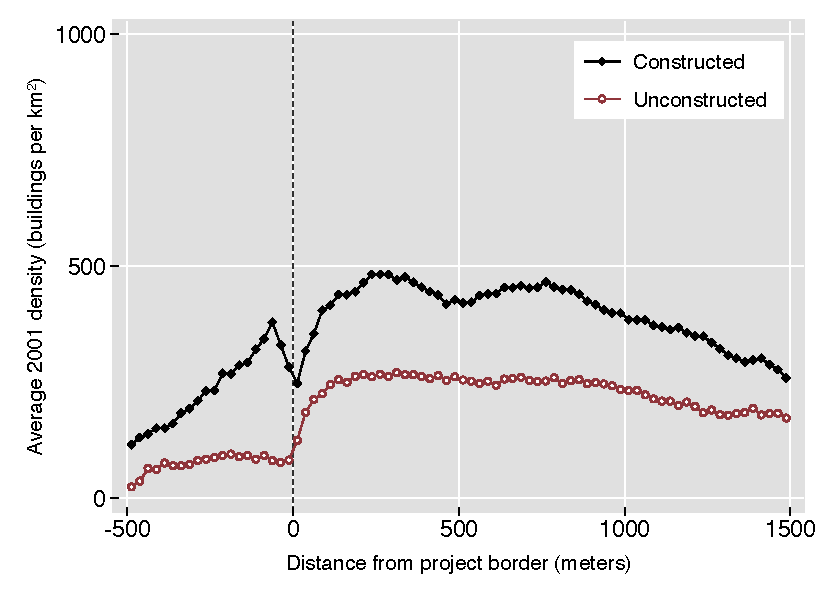
\includegraphics[width=\textwidth,trim={0.3cm .3cm 0.1cm 0cm}, clip=true]{figures/bblu_for_pre_means_4_spk.pdf}

%         \end{subfigure}
%         \hfill
%         \begin{subfigure}[b]{0.48\textwidth}  
%                     \caption[]%
%             {{\footnotesize \textbf{All Projects} pre-period informal  raw data}}      
%             \label{fig:preinf}
%             \centering 
%             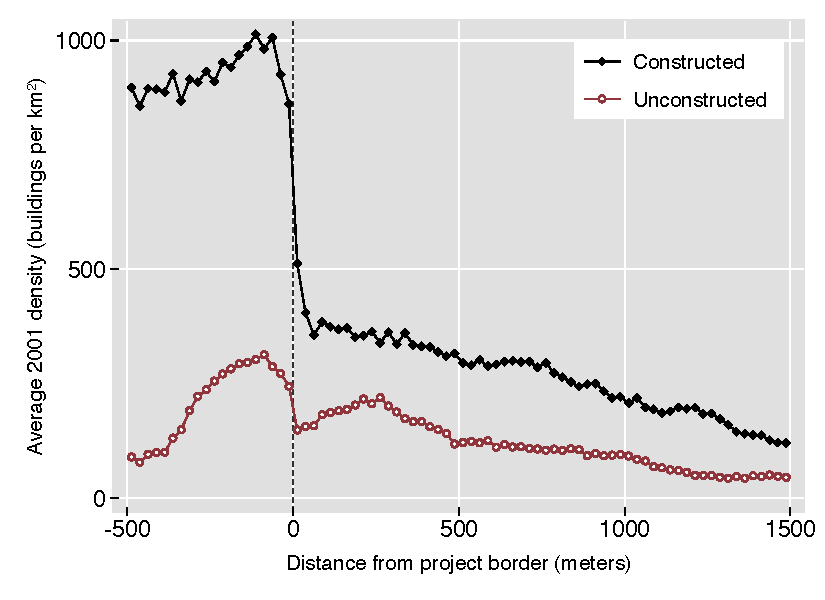
\includegraphics[width=\textwidth,trim={0.3cm .3cm 0.1cm 0cm}, clip=true]{figures/bblu_inf_pre_means_4_spk.pdf}

%         \end{subfigure}
%         \begin{subfigure}[b]{0.48\textwidth}
%                     \caption[Network2]%
%             {{\footnotesize \textbf{Greenfield} pre-period formal  raw data}}    
%             \label{fig:prefor}
%             \centering
%             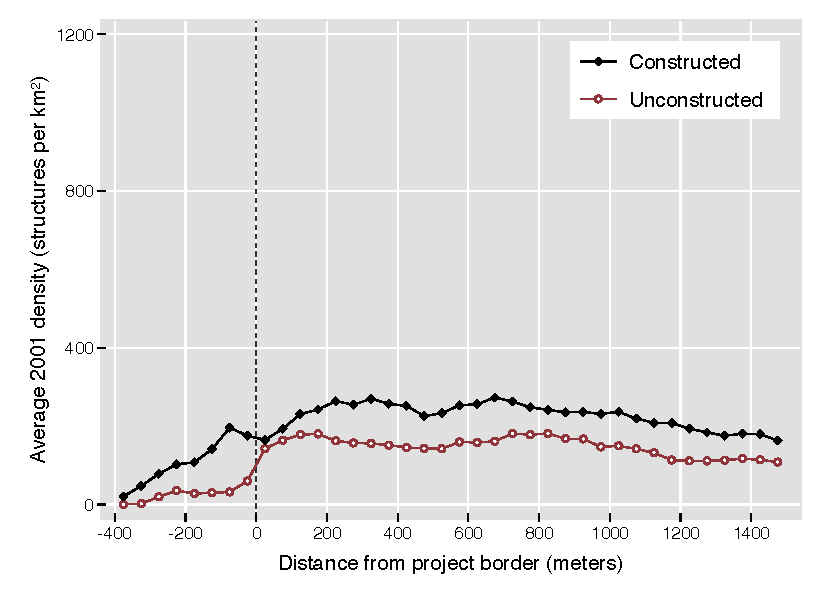
\includegraphics[width=\textwidth,trim={0.3cm .3cm 0.1cm 0cm}, clip=true]{figures/bblu_for_pre_means_4_1_spk.pdf}

%         \end{subfigure}
%         \hfill
%         \begin{subfigure}[b]{0.48\textwidth}  
%                     \caption[]%
%             {{\footnotesize \textbf{Greenfield} pre-period informal  raw data}}     
%             \label{fig:preinf}
%             \centering 
%             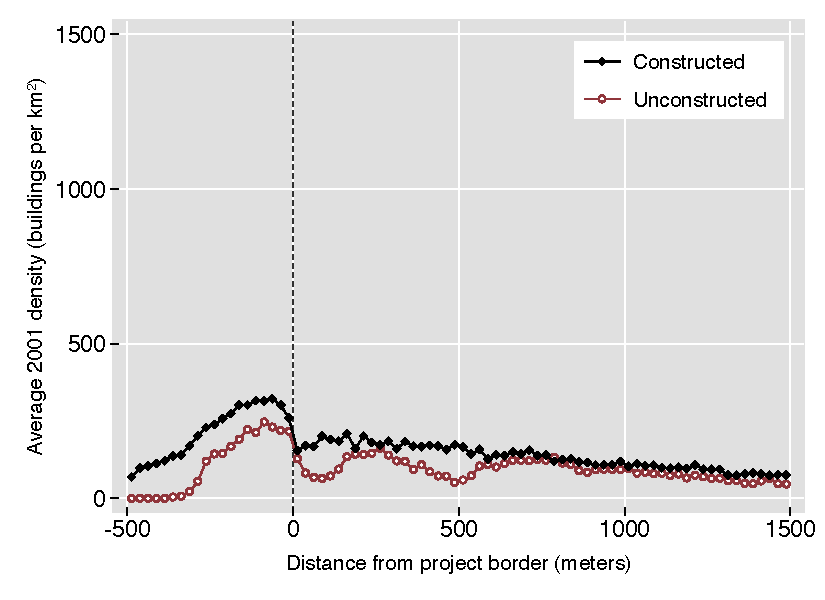
\includegraphics[width=\textwidth,trim={0.3cm .3cm 0.1cm 0cm}, clip=true]{figures/bblu_inf_pre_means_4_1_spk.pdf}

%         \end{subfigure}
%         \begin{subfigure}[b]{0.48\textwidth}
%                     \caption[Network2]%
%             {{\footnotesize \textbf{In-Situ} pre-period formal  raw data}}   
%             \label{fig:prefor}
%             \centering
%             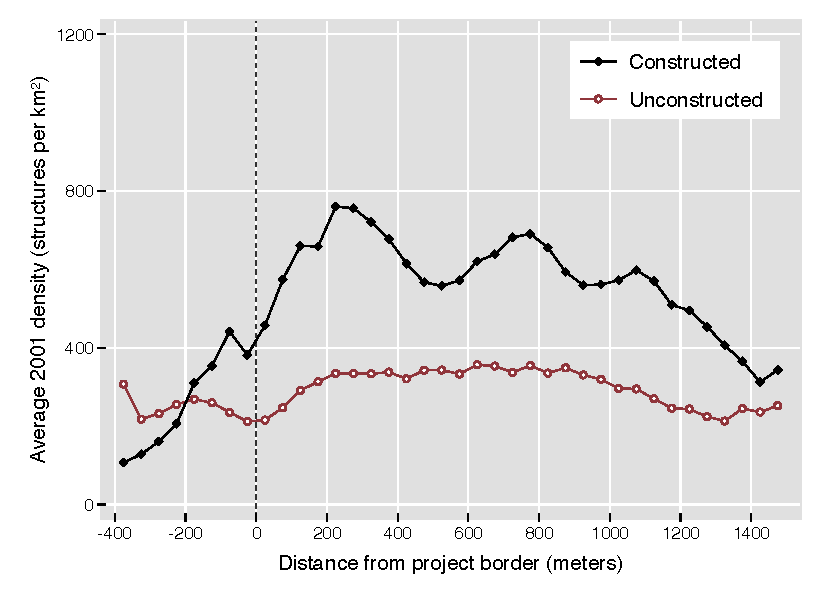
\includegraphics[width=\textwidth,trim={0.3cm .3cm 0.1cm 0cm}, clip=true]{figures/bblu_for_pre_means_4_2_spk.pdf}

%         \end{subfigure}
%         \hfill
%         \begin{subfigure}[b]{0.48\textwidth}  
%                     \caption[]%
%             {{\footnotesize \textbf{In-Situ} pre-period informal  raw data}}     
%             \label{fig:preinf}
%             \centering 
%             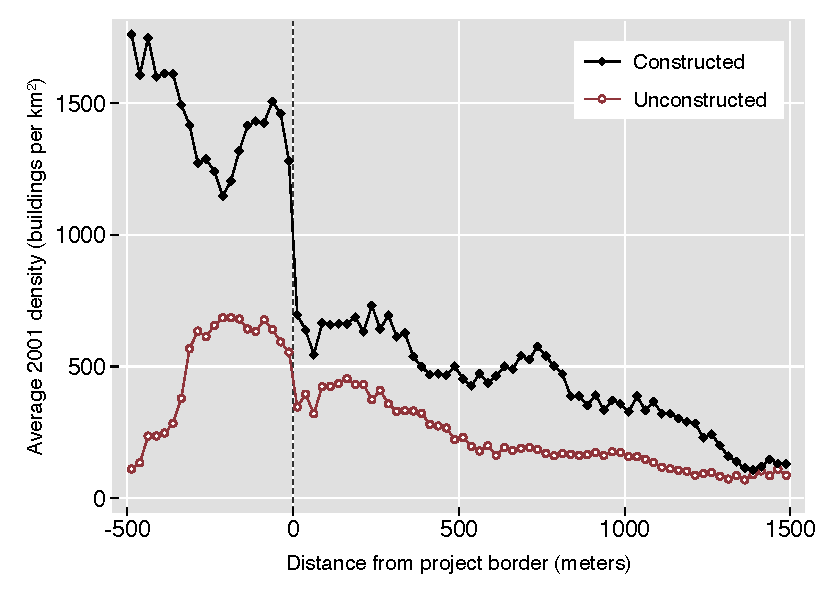
\includegraphics[width=\textwidth,trim={0.3cm .3cm 0.1cm 0cm}, clip=true]{figures/bblu_inf_pre_means_4_2_spk.pdf}

%         \end{subfigure}
%         \begin{subfigure}[b]{0.48\textwidth}
%                     \caption[Network2]%
%             {{\footnotesize \textbf{Other} pre-period formal  raw data}}   
%             \label{fig:prefor}
%             \centering
%             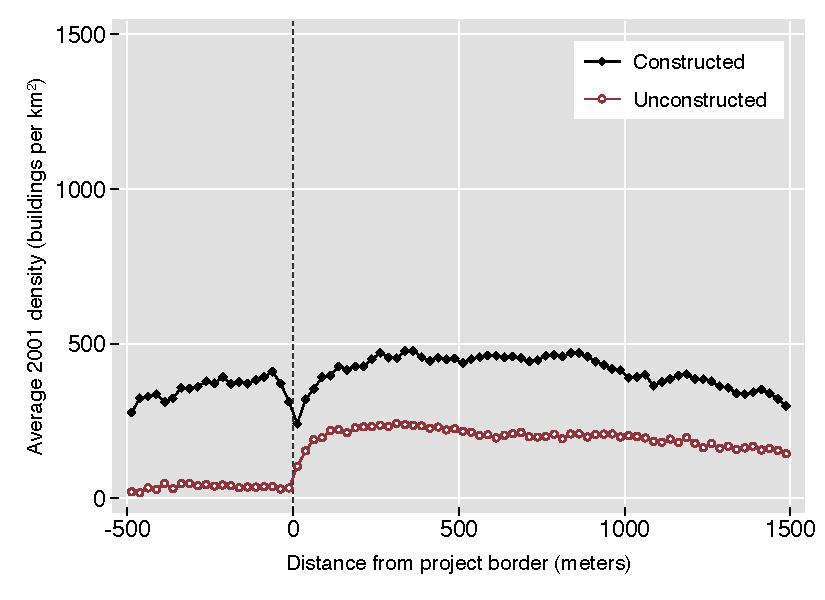
\includegraphics[width=\textwidth,trim={0.3cm .3cm 0.1cm 0cm}, clip=true]{figures/bblu_for_pre_means_4_3_spk.pdf}

%         \end{subfigure}
%         \hfill
%         \begin{subfigure}[b]{0.48\textwidth}  
%                     \caption[]%
%             {{\footnotesize \textbf{Other} pre-period informal  raw data}}      
%             \label{fig:preinf}
%             \centering 
%             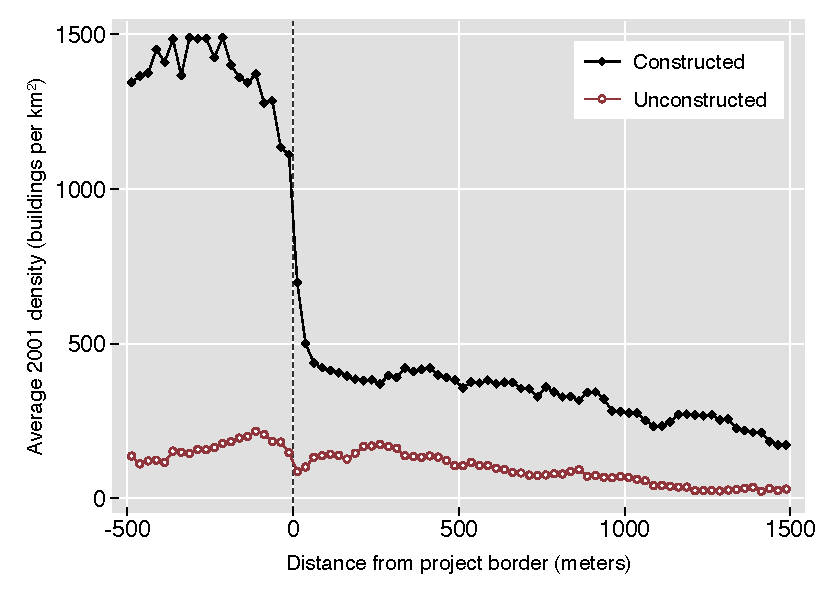
\includegraphics[width=\textwidth,trim={0.3cm .3cm 0.1cm 0cm}, clip=true]{figures/bblu_inf_pre_means_4_3_spk.pdf}

%         \end{subfigure}
% \end{figure*}








% \begin{figure*}
%         \centering
%    %     \caption[ Pre-Period Housing Densities in Constructed and Unconstructed Projects Areas ]
%   %      {\small Pre-Period Densities} 
%         %\vspace{2mm}
%         \begin{subfigure}[b]{0.48\textwidth}
%             \caption[Network2]%
%             {{\footnotesize \textbf{All Projects} changes formal raw data}}    
%             \label{fig:prefor}
%             \centering
%             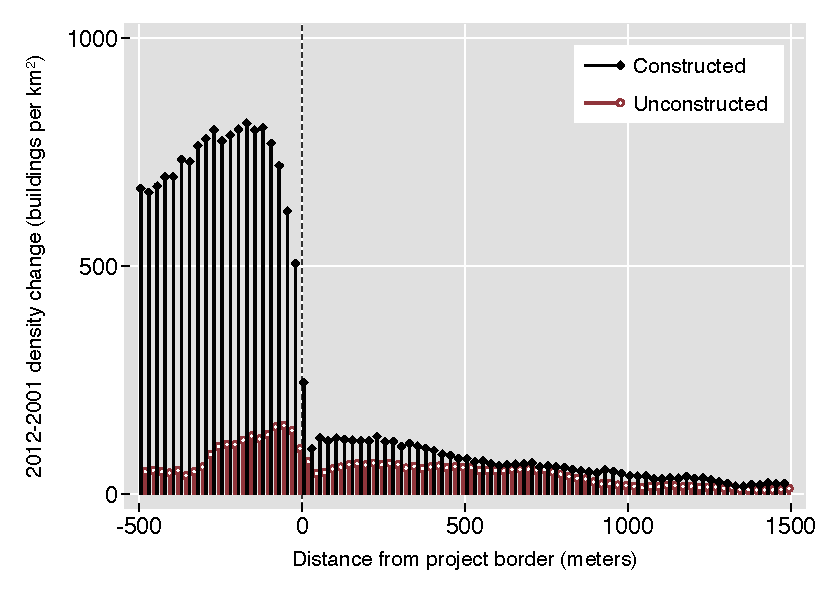
\includegraphics[width=\textwidth,trim={0.3cm .3cm 0.1cm 0cm}, clip=true]{figures/bblu_for_rawchanges_4_spk.pdf}

%         \end{subfigure}
%         \hfill
%         \begin{subfigure}[b]{0.48\textwidth}  
%                     \caption[]%
%             {{\footnotesize \textbf{All Projects} changes informal  raw data}}      
%             \label{fig:preinf}
%             \centering 
%             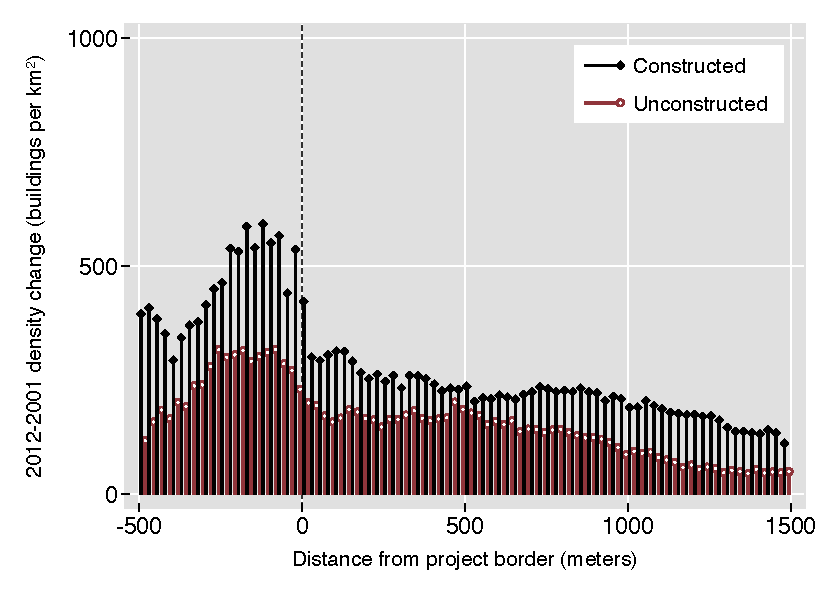
\includegraphics[width=\textwidth,trim={0.3cm .3cm 0.1cm 0cm}, clip=true]{figures/bblu_inf_rawchanges_4_spk.pdf}

%         \end{subfigure}
%         \begin{subfigure}[b]{0.48\textwidth}
%                     \caption[Network2]%
%             {{\footnotesize \textbf{Greenfield} changes formal  raw data}}    
%             \label{fig:prefor}
%             \centering
%             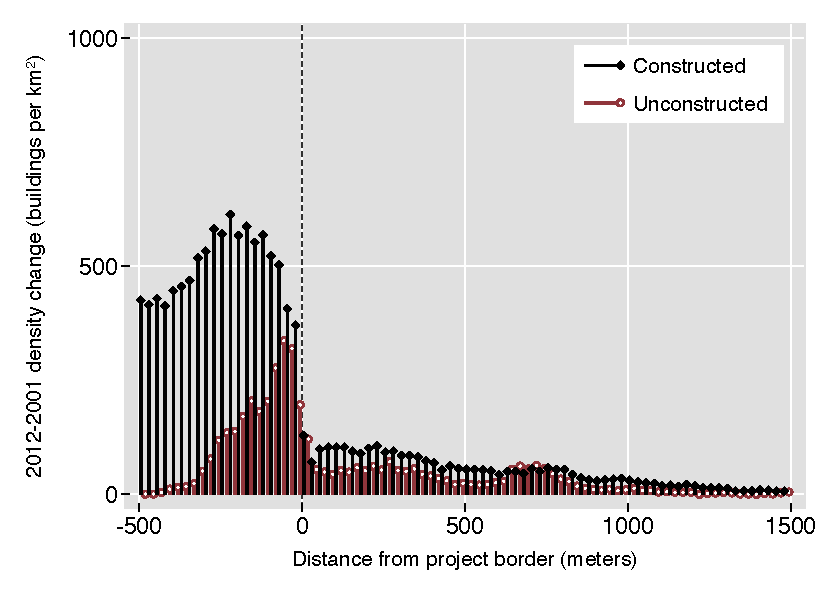
\includegraphics[width=\textwidth,trim={0.3cm .3cm 0.1cm 0cm}, clip=true]{figures/bblu_for_rawchanges_4_1_spk.pdf}

%         \end{subfigure}
%         \hfill
%         \begin{subfigure}[b]{0.48\textwidth}  
%                     \caption[]%
%             {{\footnotesize \textbf{Greenfield} changes informal raw data }}     
%             \label{fig:preinf}
%             \centering 
%             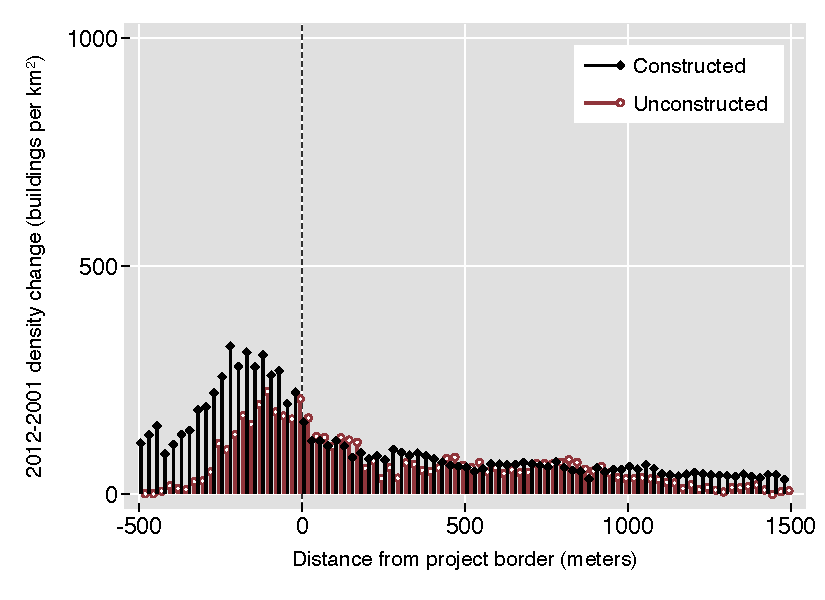
\includegraphics[width=\textwidth,trim={0.3cm .3cm 0.1cm 0cm}, clip=true]{figures/bblu_inf_rawchanges_4_1_spk.pdf}

%         \end{subfigure}
%         \begin{subfigure}[b]{0.48\textwidth}
%                     \caption[Network2]%
%             {{\footnotesize \textbf{In-Situ} changes formal raw data }}   
%             \label{fig:prefor}
%             \centering
%             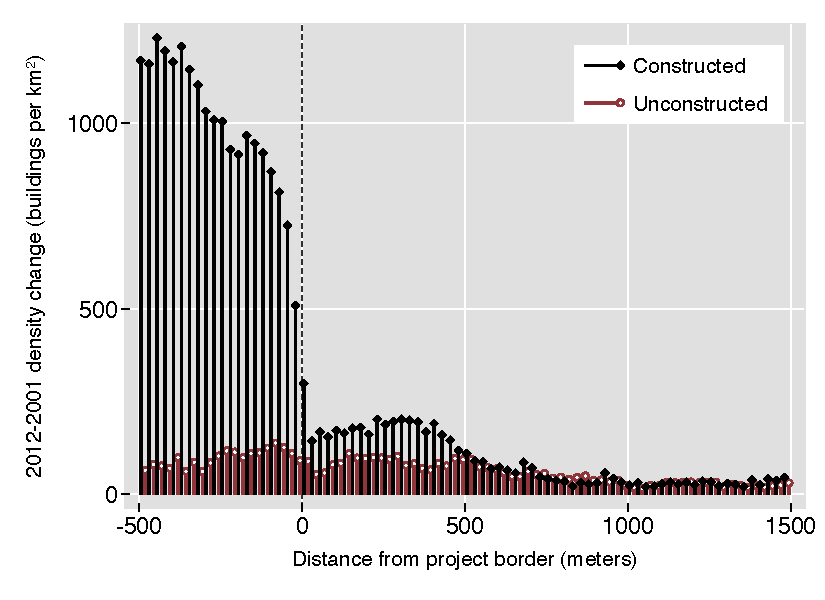
\includegraphics[width=\textwidth,trim={0.3cm .3cm 0.1cm 0cm}, clip=true]{figures/bblu_for_rawchanges_4_2_spk.pdf}

%         \end{subfigure}
%         \hfill
%         \begin{subfigure}[b]{0.48\textwidth}  
%                     \caption[]%
%             {{\footnotesize \textbf{In-Situ} changes informal raw data }}     
%             \label{fig:preinf}
%             \centering 
%             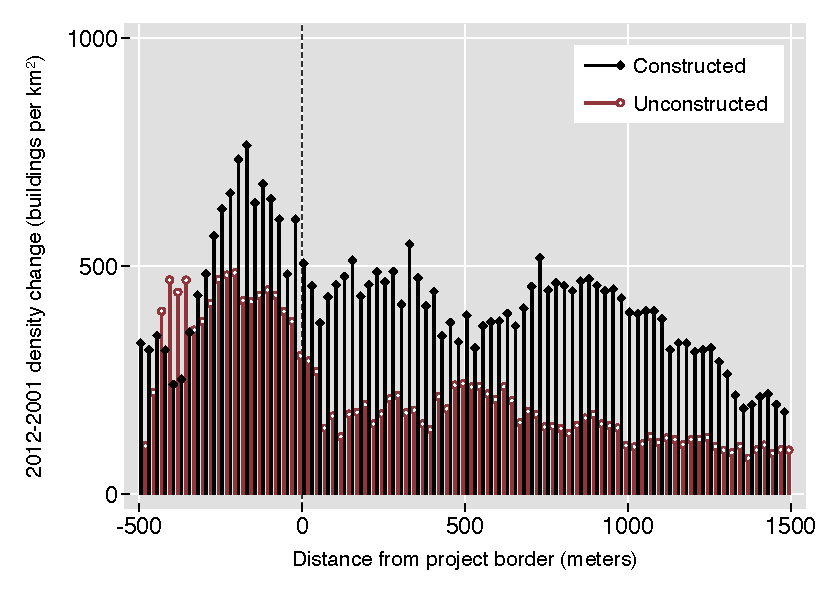
\includegraphics[width=\textwidth,trim={0.3cm .3cm 0.1cm 0cm}, clip=true]{figures/bblu_inf_rawchanges_4_2_spk.pdf}

%         \end{subfigure}
%         \begin{subfigure}[b]{0.48\textwidth}
%                     \caption[Network2]%
%             {{\footnotesize \textbf{Other} changes formal raw data}}   
%             \label{fig:prefor}
%             \centering
%             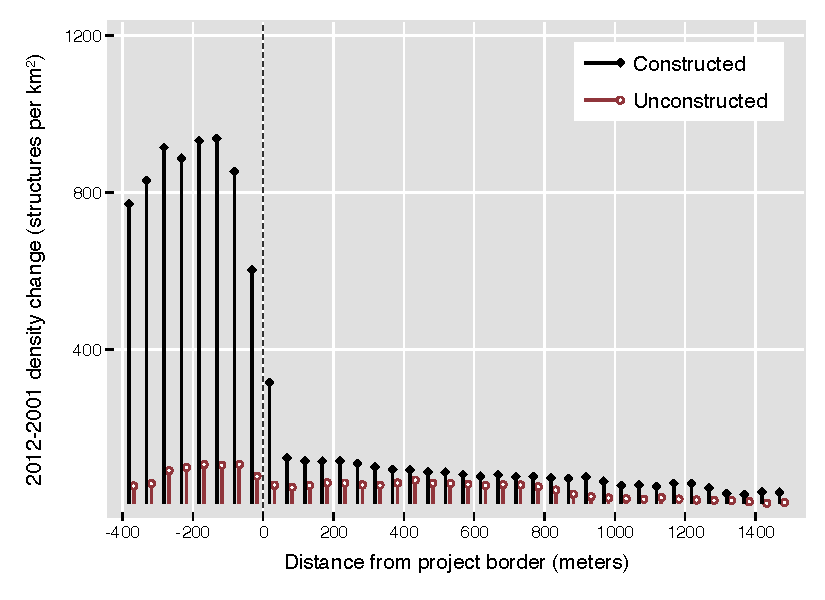
\includegraphics[width=\textwidth,trim={0.3cm .3cm 0.1cm 0cm}, clip=true]{figures/bblu_for_rawchanges_4_3_spk.pdf}

%         \end{subfigure}
%         \hfill
%         \begin{subfigure}[b]{0.48\textwidth} 
%                     \caption[]%
%             {{\footnotesize \textbf{Other} changes informal  raw data}}      
%             \label{fig:preinf} 
%             \centering 
%             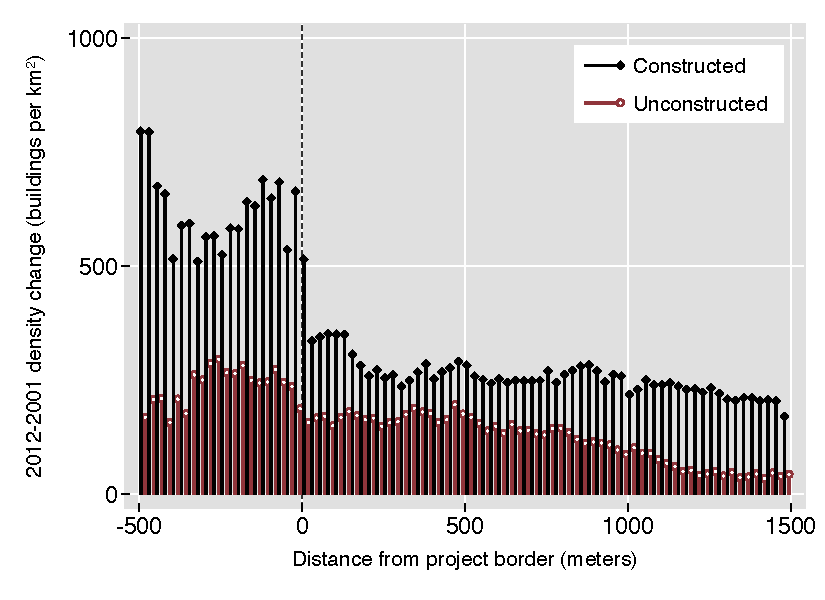
\includegraphics[width=\textwidth,trim={0.3cm .3cm 0.1cm 0cm}, clip=true]{figures/bblu_inf_rawchanges_4_3_spk.pdf}

%         \end{subfigure}
% \end{figure*}







\begin{table}
\caption{Building Density}
\begin{tabular}{lDDDDD}
\toprule
 & \small (1) & \small (2)  & \small (3) & \small (4) & \small (5) \\
 & Total & Formal  & Informal & Informal Bkyd. & Informal Non-Bkyd. \\ \midrule
\textbf{All Projects} \\inside project      &     452.140\textsuperscript{a}&     436.851\textsuperscript{a}&      15.289                   &     248.831\textsuperscript{a}&    -233.542\textsuperscript{a}\\
                    &   (141.471)                   &    (70.781)                   &   (102.224)                   &    (89.186)                   &    (71.453)                   \\[0.5em]
0-250m outside project &      23.820                   &       4.358                   &      19.461                   &     -21.954                   &      41.415                   \\
                    &    (47.943)                   &    (21.312)                   &    (40.243)                   &    (33.809)                   &    (28.425)                   \\[0.5em]
250-500m outside project &     -29.417                   &      -4.069                   &     -25.347                   &     -32.102                   &       6.755                   \\
                    &    (29.933)                   &    (13.307)                   &    (25.212)                   &    (21.025)                   &    (15.958)                   \\[0.5em]
R$^2$               &       0.442                   &       0.409                   &       0.405                   &       0.387                   &       0.346                   \\

\midrule
\textbf{Greenfield} \\   inside project      &     293.106\textsuperscript{c}&     226.130\textsuperscript{b}&      66.976                   &      98.477                   &     -31.501                   \\
                    &   (177.242)                   &   (111.345)                   &    (83.924)                   &    (80.963)                   &    (39.700)                   \\[0.01em]
0-250m outside project &     -19.058                   &     -14.600                   &      -4.458                   &     -36.968                   &      32.510                   \\
                    &    (47.668)                   &    (21.382)                   &    (35.596)                   &    (26.516)                   &    (29.062)                   \\[0.01em]
250-500m outside project &      -0.090                   &      -8.340                   &       8.251                   &     -15.255                   &      23.506                   \\
                    &    (31.500)                   &    (13.546)                   &    (24.615)                   &    (13.027)                   &    (18.785)                   \\[0.8em] 
\textbf{In-Situ Upgrading} \\   inside project      &     267.215                   &     596.654\textsuperscript{a}&    -329.439                   &      61.571                   &    -391.009                   \\
                    &   (625.673)                   &   (168.778)                   &   (511.823)                   &   (433.494)                   &   (320.832)                   \\[0.01em]
0-250m outside project &     122.750                   &      78.858                   &      43.892                   &     -61.516                   &     105.407                   \\
                    &   (244.203)                   &    (94.098)                   &   (194.920)                   &   (184.156)                   &   (120.035)                   \\[0.01em]
250-500m outside project &      57.037                   &      66.346                   &      -9.309                   &     -76.855                   &      67.546                   \\
                    &   (123.147)                   &    (47.645)                   &   (107.054)                   &    (94.932)                   &    (80.408)                   \\[0.8em]
\textbf{Other} \\   inside project      &     714.119\textsuperscript{a}&     602.858\textsuperscript{a}&     111.261                   &     463.924\textsuperscript{a}&    -352.663\textsuperscript{a}\\
                    &   (139.542)                   &    (71.828)                   &   (105.779)                   &   (104.689)                   &    (87.108)                   \\[0.01em]
0-250m outside project &      13.834                   &      15.351                   &      -1.516                   &     -21.613                   &      20.097                   \\
                    &    (64.872)                   &    (27.200)                   &    (56.438)                   &    (43.035)                   &    (37.445)                   \\[0.01em]
250-500m outside project &     -78.401\textsuperscript{c}&     -11.404                   &     -66.997\textsuperscript{c}&     -39.628                   &     -27.369                   \\
                    &    (45.892)                   &    (18.275)                   &    (39.153)                   &    (34.766)                   &    (16.796)                   \\[0.8em]
Mean Outcome 2001   &      526.22                   &      261.56                   &      264.66                   &       96.43                   &      168.23                   \\
Mean Outcome 2011   &      838.62                   &      385.14                   &      453.48                   &      286.79                   &      166.69                   \\
R$^2$               &       0.443                   &       0.411                   &       0.406                   &       0.388                   &       0.347                   \\
N                   &   1,705,534                   &   1,705,534                   &   1,705,534                   &   1,705,534                   &   1,705,534                   \\

\bottomrule
\end{tabular}
\end{table}





\begin{table}[h!] 
\caption{Effect of Housing Projects on Socio-demographics}
\label{table:sorting}
\small
\centering
%\caption{Census Composition Estimates }
\vspace{-2mm}
\begin{tabular}{lDDDDD}
\toprule
& \small (1) & \small (2) & \small (3) & \small (4)& \small (5)\\
& \small Age & \small P.O.B. not Gauteng & \small Unemployed & \small Years of Education & \small Monthly Income \\ \midrule 
\textbf{All Projects} \\inside project      &      -0.163                   &       0.006                   &      -0.045\textsuperscript{b}&       0.160                   &     712.957                   \\
                    &     (0.400)                   &     (0.023)                   &     (0.021)                   &     (0.162)                   &   (557.409)                   \\[0.5em]
0-250m outside project &       0.120                   &      -0.006                   &      -0.027                   &       0.125                   &     160.451                   \\
                    &     (0.313)                   &     (0.017)                   &     (0.019)                   &     (0.126)                   &   (382.409)                   \\[0.5em]
250-500m outside project &      -0.079                   &       0.008                   &      -0.015                   &      -0.073                   &    -104.838                   \\
                    &     (0.304)                   &     (0.016)                   &     (0.020)                   &     (0.112)                   &   (427.692)                   \\[0.5em]
R$^2$               &       0.703                   &       0.771                   &       0.529                   &       0.692                   &       0.666                   \\

\midrule
\textbf{Greenfield} \\   inside project      &      -0.406                   &      -0.009                   &       0.027                   &       0.576\textsuperscript{c}&    1351.726                   \\
                    &     (0.687)                   &     (0.060)                   &     (0.049)                   &     (0.320)                   &  (1012.025)                   \\[0.01em]
0-250m outside project &      -0.094                   &       0.034                   &       0.028                   &       0.060                   &     681.286                   \\
                    &     (0.743)                   &     (0.032)                   &     (0.049)                   &     (0.212)                   &   (654.991)                   \\[0.01em]
250-500m outside project &      -0.775                   &       0.039                   &       0.046                   &       0.208                   &     466.483                   \\
                    &     (0.923)                   &     (0.033)                   &     (0.050)                   &     (0.272)                   &   (656.186)                   \\[0.8em] 
\textbf{In-Situ Upgrading} \\   inside project      &       0.768                   &       0.068\textsuperscript{c}&      -0.071\textsuperscript{b}&      -0.090                   &    -325.539                   \\
                    &     (0.588)                   &     (0.041)                   &     (0.028)                   &     (0.353)                   &   (933.925)                   \\[0.01em]
0-250m outside project &       0.227                   &      -0.001                   &      -0.039                   &       0.078                   &    -341.246                   \\
                    &     (0.349)                   &     (0.029)                   &     (0.035)                   &     (0.277)                   &   (831.050)                   \\[0.01em]
250-500m outside project &       0.138                   &       0.006                   &      -0.055\textsuperscript{b}&      -0.168                   &   -1311.012                   \\
                    &     (0.350)                   &     (0.029)                   &     (0.027)                   &     (0.235)                   &  (1076.414)                   \\[0.8em]
\textbf{Other} \\   inside project      &      -0.260                   &      -0.019                   &      -0.053\textsuperscript{c}&       0.149                   &     907.983                   \\
                    &     (0.502)                   &     (0.034)                   &     (0.029)                   &     (0.200)                   &   (774.648)                   \\[0.01em]
0-250m outside project &       0.237                   &      -0.014                   &      -0.038                   &       0.087                   &      43.901                   \\
                    &     (0.451)                   &     (0.026)                   &     (0.024)                   &     (0.152)                   &   (550.678)                   \\[0.01em]
250-500m outside project &       0.188                   &      -0.002                   &      -0.023                   &      -0.164                   &     183.286                   \\
                    &     (0.419)                   &     (0.024)                   &     (0.024)                   &     (0.140)                   &   (532.373)                   \\[0.8em]
Mean Outcome 2001   &       27.30                   &        0.37                   &        0.47                   &        8.27                   &    2,477.01                   \\
Mean Outcome 2011   &       28.30                   &        0.43                   &        0.33                   &        9.68                   &    4,486.48                   \\
R$^2$               &       0.706                   &       0.774                   &       0.530                   &       0.695                   &       0.669                   \\
N                   &      12,734                   &      12,727                   &      12,724                   &      12,728                   &      12,724                   \\

\bottomrule
\multicolumn{6}{l}{\footnotesize Standard errors clustered at the project level in parenthesis. \textsuperscript{c} p$<$0.10, \textsuperscript{b} p$<$0.05, \textsuperscript{a} p$<$0.01  }\\
\multicolumn{6}{l}{\footnotesize P.O.B. means ``place of birth.''  Monthly income is in Rands.}
\end{tabular}
\end{table}








\begin{landscape}
{\footnotesize

\begin{table}[]
\small
\centering
\caption{Census Household-level Estimates }\label{table:censusestimates}
\vspace{-2mm}
\resizebox{.9\linewidth}{!}{
\begin{tabular}{lDDDDDDDD}
\toprule
 & \small (1) & \small (2)  & \small (3) & \small (4) & \small (5)  & \small (6)  & \small (7) & (8)\\
 & \small Flush Toilet & \small Water Indoors  & \small Electricity Cooking & \small Electricity Heating & \small Electricity Lighting  & \small Number of Rooms  & \small Household Size & Population Density\\ \midrule 
\textbf{All Projects} \\inside project      &       0.073                   &       0.159\textsuperscript{a}&       0.119\textsuperscript{c}&       0.093                   &       0.074                   &       0.199                   &       0.058                   &   -1075.527                   \\
                    &     (0.055)                   &     (0.051)                   &     (0.062)                   &     (0.061)                   &     (0.067)                   &     (0.208)                   &     (0.087)                   &  (1001.543)                   \\[0.5em]
0-250m outside project &      -0.000                   &       0.084\textsuperscript{c}&      -0.011                   &      -0.016                   &      -0.019                   &       0.059                   &      -0.051                   &    -931.449                   \\
                    &     (0.036)                   &     (0.044)                   &     (0.039)                   &     (0.038)                   &     (0.040)                   &     (0.146)                   &     (0.065)                   &  (1103.531)                   \\[0.5em]
250-500m outside project &      -0.025                   &       0.010                   &      -0.009                   &      -0.006                   &      -0.018                   &      -0.045                   &      -0.041                   &   -1160.158                   \\
                    &     (0.029)                   &     (0.037)                   &     (0.027)                   &     (0.028)                   &     (0.026)                   &     (0.127)                   &     (0.057)                   &  (1300.794)                   \\[0.5em]
R$^2$               &       0.615                   &       0.593                   &       0.668                   &       0.634                   &       0.638                   &       0.676                   &       0.691                   &       0.607                   \\

\midrule
\textbf{Greenfield} \\   inside project      &       0.143                   &       0.128                   &       0.203                   &       0.088                   &       0.169                   &       0.700\textsuperscript{c}&       0.003                   &     -37.386                   \\
                    &     (0.143)                   &     (0.145)                   &     (0.131)                   &     (0.149)                   &     (0.130)                   &     (0.384)                   &     (0.206)                   &  (2372.927)                   \\[0.01em]
0-250m outside project &       0.029                   &       0.105                   &       0.008                   &      -0.005                   &      -0.027                   &       0.327                   &       0.134                   &   -2253.949                   \\
                    &     (0.077)                   &     (0.097)                   &     (0.057)                   &     (0.063)                   &     (0.065)                   &     (0.300)                   &     (0.155)                   &  (2266.995)                   \\[0.01em]
250-500m outside project &      -0.048                   &      -0.065                   &      -0.017                   &       0.029                   &      -0.018                   &      -0.023                   &      -0.042                   &   -5835.768                   \\
                    &     (0.073)                   &     (0.068)                   &     (0.062)                   &     (0.066)                   &     (0.052)                   &     (0.287)                   &     (0.101)                   &  (4558.272)                   \\[0.8em] 
\textbf{In-Situ Upgrading} \\   inside project      &       0.034                   &       0.097                   &       0.004                   &       0.045                   &      -0.108                   &      -0.151                   &      -0.073                   &   -2221.341                   \\
                    &     (0.112)                   &     (0.087)                   &     (0.129)                   &     (0.110)                   &     (0.135)                   &     (0.327)                   &     (0.146)                   &  (1636.523)                   \\[0.01em]
0-250m outside project &       0.051                   &       0.043                   &      -0.043                   &      -0.066                   &      -0.061                   &      -0.215                   &      -0.076                   &   -1636.726                   \\
                    &     (0.085)                   &     (0.083)                   &     (0.083)                   &     (0.077)                   &     (0.084)                   &     (0.235)                   &     (0.119)                   &  (1897.087)                   \\[0.01em]
250-500m outside project &       0.015                   &       0.058                   &       0.022                   &       0.004                   &      -0.016                   &      -0.294                   &      -0.033                   &     576.408                   \\
                    &     (0.057)                   &     (0.073)                   &     (0.055)                   &     (0.055)                   &     (0.060)                   &     (0.228)                   &     (0.095)                   &  (1270.819)                   \\[0.8em]
\textbf{Other} \\   inside project      &       0.060                   &       0.186\textsuperscript{a}&       0.140\textsuperscript{c}&       0.104                   &       0.137                   &       0.194                   &       0.138                   &    -469.730                   \\
                    &     (0.073)                   &     (0.064)                   &     (0.085)                   &     (0.087)                   &     (0.089)                   &     (0.298)                   &     (0.116)                   &  (1157.858)                   \\[0.01em]
0-250m outside project &      -0.057                   &       0.096                   &      -0.030                   &      -0.015                   &      -0.025                   &       0.059                   &      -0.109                   &    -207.145                   \\
                    &     (0.046)                   &     (0.060)                   &     (0.052)                   &     (0.051)                   &     (0.054)                   &     (0.199)                   &     (0.082)                   &  (1259.370)                   \\[0.01em]
250-500m outside project &      -0.037                   &       0.019                   &      -0.012                   &      -0.013                   &      -0.011                   &       0.053                   &      -0.069                   &    -600.224                   \\
                    &     (0.033)                   &     (0.051)                   &     (0.035)                   &     (0.037)                   &     (0.035)                   &     (0.177)                   &     (0.087)                   &   (845.267)                   \\[0.8em]
Mean Outcome 2001   &        0.79                   &        0.35                   &        0.66                   &        0.62                   &        0.77                   &        3.30                   &        3.51                   &    8,566.83                   \\
Mean Outcome 2011   &        0.83                   &        0.54                   &        0.81                   &        0.72                   &        0.82                   &        3.56                   &        3.18                   &    9,823.82                   \\
R$^2$               &       0.626                   &       0.603                   &       0.675                   &       0.640                   &       0.645                   &       0.681                   &       0.694                   &       0.609                   \\
N                   &      12,732                   &      12,732                   &      12,732                   &      12,732                   &      12,732                   &      12,709                   &      12,730                   &      12,734                   \\

\bottomrule
\multicolumn{9}{l}{\footnotesize All regressions include 3km grid Fixed-Effects. Standard errors clustered at the project level in parenthesis. \textsuperscript{c} p$<$0.10,\textsuperscript{b} p$<$0.05,\textsuperscript{a} p$<$0.01 }
\end{tabular}
}
\end{table}

}
\end{landscape}




\begin{table}
\small
\centering
\caption{Triple Difference Estimates on Log-Prices}\label{table:priceDDD_het}
\vspace{-2mm}
\begin{tabular}{lCC}
\toprule
 & \small (1) & \small (2)  \\ \midrule 
 \textbf{All Projects} \\
 inside project      &      -0.165                   &      -0.150                   \\
                    &     (0.273)                   &     (0.268)                   \\[0.55em]
0-250m outside project &      -0.024                   &      -0.017                   \\
                    &     (0.069)                   &     (0.069)                   \\[0.5em]
250-500m outside project &      -0.008                   &      -0.002                   \\
                    &     (0.053)                   &     (0.053)                   \\[0.5em]
Lot Size Controls   &                               &  \checkmark                   \\
r2                  &        0.52                   &        0.52                   \\
N                   &      67,751                   &      67,751                   \\

 \midrule
\textbf{Greenfield} \\   inside project      &       0.075                   &      -0.054                   \\
                    &     (0.235)                   &     (0.231)                   \\[0.01em]
0-250m outside project &       0.121                   &       0.135                   \\
                    &     (0.201)                   &     (0.195)                   \\[0.01em]
250-500m outside project &      -0.147                   &      -0.146                   \\
                    &     (0.127)                   &     (0.128)                   \\[0.8em]
\textbf{In-Situ Upgrading} \\   inside project      &       0.065                   &       0.126                   \\
                    &     (0.333)                   &     (0.303)                   \\[0.01em]
0-250m outside project &      -0.196\textsuperscript{c}&      -0.194\textsuperscript{c}\\
                    &     (0.112)                   &     (0.110)                   \\[0.01em]
250-500m outside project &      -0.022                   &      -0.019                   \\
                    &     (0.087)                   &     (0.089)                   \\[0.8em]
\textbf{Other} \\   inside project      &      -0.330                   &      -0.287                   \\
                    &     (0.329)                   &     (0.321)                   \\[0.01em]
0-250m outside project &       0.037                   &       0.041                   \\
                    &     (0.086)                   &     (0.086)                   \\[0.01em]
250-500m outside project &      -0.014                   &      -0.009                   \\
                    &     (0.084)                   &     (0.082)                   \\[0.8em]
Lot Size Controls   &                               &  \checkmark                   \\
r2                  &        0.52                   &        0.52                   \\
N                   &      67,751                   &      67,751                   \\

\bottomrule
\multicolumn{3}{l}{\footnotesize Standard errors clustered at the project level in parenthesis.} \\
\multicolumn{3}{l}{ \textsuperscript{c} p$<$0.10,\textsuperscript{b} p$<$0.05,\textsuperscript{a} p$<$0.01 }
\end{tabular}
\end{table} 

% \begin{figure}
% 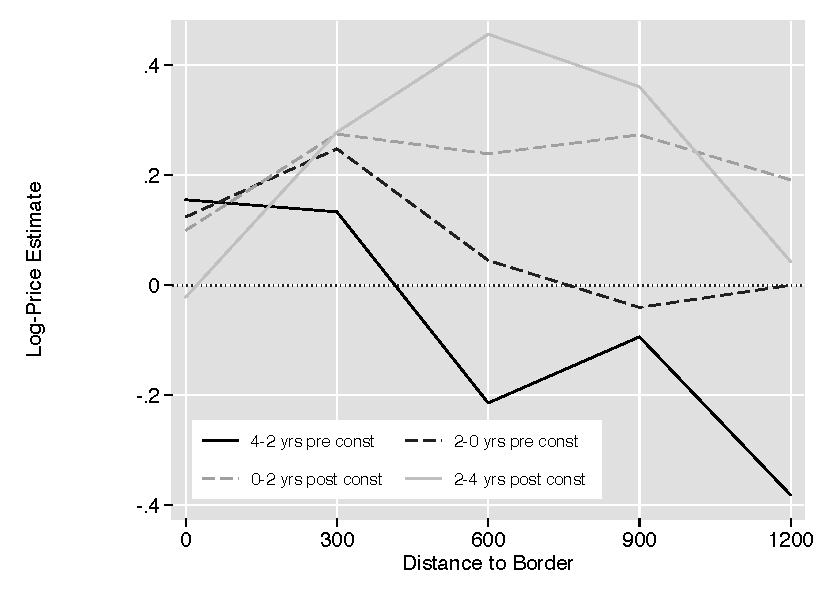
\includegraphics{figures/price_to_event_30.pdf}
% \end{figure}


\end{document}


